\documentclass[12pt]{article}
\usepackage[utf8]{inputenc}
\usepackage{graphicx}
\usepackage{booktabs}
\usepackage[margin=1in]{geometry}
\usepackage{amsmath}
\usepackage{amssymb}
\usepackage{enumitem}
\usepackage{caption}
\usepackage{titlesec}
\usepackage{xcolor}
\usepackage{fancyhdr}
\usepackage{microtype}
\usepackage{listings}
\usepackage{framed}
\usepackage{multirow}
\usepackage{float}
\usepackage{makecell}
\usepackage{array}
\usepackage{tabularx}
\usepackage{hyperref}
\usepackage{tikz}
\usetikzlibrary{arrows.meta, positioning, backgrounds, fit, shapes.geometric, calc}
\usepackage{times}  % Times New Roman font

% Code styling for C / Embedded C
\definecolor{codegreen}{rgb}{0,0.55,0}
\definecolor{codegray}{rgb}{0.45,0.45,0.45}
\definecolor{codepurple}{rgb}{0.58,0,0.82}
\definecolor{codeblue}{rgb}{0.05,0.2,0.7}
\definecolor{backcolour}{rgb}{0.97,0.97,0.96}

\lstdefinestyle{cstyle}{
    language=C,
    backgroundcolor=\color{backcolour},
    basicstyle=\ttfamily\footnotesize,
    keywordstyle=\color{codeblue}\bfseries,
    commentstyle=\color{codegreen}\itshape,
    stringstyle=\color{codepurple},
    numberstyle=\tiny\color{codegray},
    numbers=left,
    stepnumber=1,
    numbersep=7pt,
    tabsize=2,
    showstringspaces=false,
    breaklines=true,
    breakatwhitespace=true,
    frame=single,
    captionpos=b,
}
\lstset{style=cstyle}

% Geometry Setup with sufficient headheight for fancyhdr
\geometry{a4paper, margin=1in, headheight=15pt}

% Title Formatting with section numbering
\titleformat{\section}{\normalfont\Large\bfseries\color{black}}{\thesection}{1em}{}
\titleformat{\subsection}{\normalfont\large\bfseries\color{black}}{\thesubsection}{1em}{}
\titleformat{\subsubsection}{\normalfont\normalsize\bfseries\color{black}}{\thesubsubsection}{1em}{}

% Command for first page border
\newcommand{\firstpageborder}{
    \begin{tikzpicture}[remember picture, overlay]
        \draw[line width=2.5pt, black] 
            ([xshift=15mm, yshift=-10mm]current page.north west) 
            rectangle 
            ([xshift=-15mm, yshift=10mm]current page.south east);
    \end{tikzpicture}
}

\begin{document}

% =========================================================================
% COVER PAGE
% =========================================================================
\thispagestyle{empty}
\firstpageborder

\begin{center}
    \vspace*{-0.5em}
    {\bfseries\large VIETNAM NATIONAL UNIVERSITY, HO CHI MINH CITY}\\[0.3em]
    {\bfseries\large HO CHI MINH CITY UNIVERSITY OF TECHNOLOGY}\\[0.3em]
    {\bfseries\normalsize FACULTY OF COMPUTER SCIENCE AND ENGINEERING}\\[1.5em]
    
\includegraphics[width=0.22\textwidth]{hcmut.png}
    \vspace{1.8em}

    {\Large\textbf{EMBEDDED SYSTEMS (CO3053)}}\\[0.5em]
    {\large\textbf{Assignment 2: State Machine and Flowchart Design}}\\[0.8em]
    \rule{0.88\textwidth}{0.8pt}\\[0.8em]
    {\LARGE\textbf{Automated Washing Machine}}\\[0.3em]
    {\LARGE\textbf{Control Unit}}\\[0.6em]
    {\normalsize\textit{Extended Finite State Machine Modeling, Flowchart Synthesis, and Firmware Implementation}}\\[0.6em]
    \rule{0.88\textwidth}{0.8pt}
    \vspace{2.2em}

    \begin{minipage}{0.65\textwidth}
        \begin{flushleft}
            \textbf{Instructor:} Dr. Pham Hoang Anh \\
            \textbf{Students:} \\
            \hspace*{1em} Le Thanh Binh - 2352118 \\
            \hspace*{1em} Pham Hong Minh Tu - 2353293 \\
            \hspace*{1em} Pham Minh Nhat - 2352863\\
            \textbf{Class:} CC02
        \end{flushleft}
    \end{minipage}
    \vfill
    {\normalsize HO CHI MINH CITY, October 2026}
    \vspace*{0.5em}
\end{center}

% =========================================================================
% HEADER / FOOTER & ABSTRACT
% =========================================================================
\clearpage
\pagestyle{fancy}
\fancyhead[L]{\slshape\footnotesize CO3053 -- Embedded Systems: Assignment 2}
\fancyhead[R]{\slshape\footnotesize Washing Machine Control Unit}
\renewcommand{\headrulewidth}{0.4pt}
\fancyfoot[C]{}
\fancyfoot[R]{\color{black}Page \thepage}
\pagenumbering{roman}

\begin{abstract}
This engineering report presents the rigorous formal modeling, architectural design, and embedded firmware implementation of an automated washing machine control unit, conforming directly to the theoretical principles delivered in \textbf{Lecture~4 (State Machine and Flowchart)}. The system is governed by a multi-button user interface (\texttt{STOP}, \texttt{RUN}, \texttt{PAUSE}), a coin acceptance mechanism (strictly processing 10-cent, 20-cent, and 50-cent denominations), two diagnostic indicator LEDs (Red LED and Blue LED), and a washing motor actuator. To satisfy complex behavioral requirements—including a 50-cent activation threshold without redundancy refunds, a non-pausing 30-minute wash timer during operational suspension, an error-handling super-state, and a double-press emergency stop mechanism—the controller is formulated as an \textbf{Extended Finite State Machine (EFSM)}. 

Outputs are synthesized under the \textbf{Moore machine model} to guarantee glitch-free, stable signaling for optical and mechanical actuators. Algorithmic components, including non-blocking software timers, $20\,\text{ms}$ contact debouncing, and pulse-frequency LED toggling, are systematically structured via standard flowcharts. The complete control unit is realized in modular C targeting an ARM Cortex-M3 microcontroller (\texttt{STM32F103C8T6}) and validated in the Proteus~8 Professional virtual system modeling environment. Comprehensive state and transition coverage matrices substantiate the deterministic correctness, fault-tolerance, and robustness of the proposed architecture.
\end{abstract}

\vspace{0.8cm}
\tableofcontents
\newpage

\pagenumbering{arabic}
\setcounter{page}{1}

% =========================================================================
% SECTION 1: INTRODUCTION & PROBLEM FORMULATION
% =========================================================================
\section{Introduction and Problem Formulation}

\subsection{System Functional Requirements}
The design target is a robust, fail-safe control unit for a commercial coin-operated washing machine. According to the specification sheet, the system must satisfy the following explicit operational criteria:
\begin{enumerate}[label=\textbf{R\arabic*.}]
    \item \textbf{User Inputs:} The machine is manipulated via three momentary push buttons: \texttt{STOP}, \texttt{RUN}, and \texttt{PAUSE}.
    \item \textbf{Visual Telemetry (LEDs):} Visual feedback is provided by a Red LED (\texttt{RLED}) and a Blue LED (\texttt{BLED}):
    \begin{itemize}
        \item \texttt{RLED} is continuously \textbf{ON} when the machine is in standby (available to serve).
        \item \texttt{RLED} is \textbf{BLINKING} ($1\,\text{Hz}$, $500\,\text{ms}$ period) when an internal fault or error is detected.
        \item \texttt{BLED} is continuously \textbf{ON} when sufficient credit has been deposited and the machine is ready to execute.
        \item \texttt{BLED} is \textbf{BLINKING} ($1\,\text{Hz}$) while the washing cycle is actively running.
    \end{itemize}
    \item \textbf{Monetary Validation and Clearing:} The unit accepts exclusively 10-cent, 20-cent, and 50-cent coins. The washing operation is strictly prohibited until at least 50~cents has been accumulated. Once credit satisfies $\text{Credit} \ge 50\,\text{cents}$, pressing \texttt{RUN} activates the cycle, instantly clearing the deposited balance without returning surplus change (redundancies).
    \item \textbf{Washing Cycle and Temporal Continuity:} The execution phase is governed by a 30-minute ($1{,}800\,\text{s}$) countdown timer. Pressing \texttt{PAUSE} halts drum agitation, but \textbf{the 30-minute timer continues counting down uninterrupted}. Pressing \texttt{RUN} resumes agitation.
    \item \textbf{Cycle Termination and Forced Stop:} The machine terminates automatically once the 30-minute countdown reaches zero. Alternatively, pressing \texttt{STOP} \textbf{twice in succession} executes an emergency forced stop, immediately halting actuators and returning the unit to standby.
\end{enumerate}

\subsection{Theoretical Principles from Lecture 4}
Lecture~4 emphasizes that complex embedded systems cannot be reliably constructed using ad-hoc branching. Instead, a disciplined design framework must be maintained:
\begin{itemize}
    \item \textbf{Moore vs. Mealy Formulation (Slide~6):} In a Moore machine, outputs depend purely on the active state:
    \begin{equation}
        \mathbf{Y}(t) = \lambda(\mathbf{S}(t))
    \end{equation}
    whereas in a Mealy machine, outputs depend on both state and instantaneous inputs:
    \begin{equation}
        \mathbf{Y}(t) = \lambda(\mathbf{S}(t), \mathbf{X}(t))
    \end{equation}
    Slide~6 establishes the foundational rule of thumb: \textit{prefer Moore for outputs that must be clean and stable (such as LEDs and motor drivers); prefer Mealy only when instantaneous input reaction is mandated}. Thus, a Moore architecture is selected to preclude actuator glitches.
    \item \textbf{Extended State Machine (Slide~22):} Pure state machines suffer from exponential state explosion when tracking numerical values. By augmenting the model with auxiliary variables (e.g., deposited coins, temporal countdowns, and button press counters), variables serve as guard conditions alongside discrete events:
    \begin{equation}
        \text{Transition: } \mathbf{S}_i \xrightarrow{\text{Event } [\text{Guard}]} \mathbf{S}_j
    \end{equation}
    \item \textbf{Mitigation of Design Pitfalls (Slide~17):} To prevent undefined behavior, the state diagram must resolve missing transitions, eliminate unreachable states, prevent non-deterministic branches, and address ambiguous direct transitions through intermediate transition confirmation states (analogous to the \texttt{Half-Open} state in the garage door study).
    \item \textbf{Flowchart vs. State Machine Complementarity (Slide~26):} A state machine models long-running, reactive event-driven behavior, whereas a flowchart models step-by-step deterministic algorithms that execute to completion within a single evaluation cycle.
\end{itemize}

% =========================================================================
% SECTION 2: HARDWARE ARCHITECTURE & CIRCUIT DESIGN
% =========================================================================
\section{Hardware Subsystem Architecture}

\subsection{Microcontroller Selection and Pin Allocation}
The controller is targeted to the \textbf{STM32F103C8T6} microcontroller (ARM 32-bit Cortex-M3 core, $72\,\text{MHz}$ maximum frequency, $64\,\text{KB}$ Flash, $20\,\text{KB}$ SRAM). The hardware pin assignment is designed for modularity, utilizing Port~A for digital sensing and Port~B for actuator control. All push buttons utilize active-low logic supported by the internal programmable weak pull-up resistors ($R_{\text{PU}} \approx 40\,\text{k}\Omega$), eliminating external discrete pull-up networks.

\begin{table}[H]
\centering
\small
\renewcommand{\arraystretch}{1.25}
\begin{tabularx}{\textwidth}{l c l l X}
\toprule
\textbf{Pin} & \textbf{LQFP48} & \textbf{I/O Mode} & \textbf{Peripheral / Net} & \textbf{Functional Description} \\
\midrule
\texttt{PA0} & Pin 10 & Input Pull-Up   & \texttt{BTN\_STOP}     & Push button to request pause/double-stop \\
\texttt{PA1} & Pin 11 & Input Pull-Up   & \texttt{BTN\_RUN}      & Push button to initiate or resume wash \\
\texttt{PA2} & Pin 12 & Input Pull-Up   & \texttt{BTN\_PAUSE}    & Push button to suspend wash cycle \\
\texttt{PA3} & Pin 13 & Input Pull-Up   & \texttt{BTN\_COIN10}   & Coin acceptor pulse: 10-cent deposit \\
\texttt{PA4} & Pin 14 & Input Pull-Up   & \texttt{BTN\_COIN20}   & Coin acceptor pulse: 20-cent deposit \\
\texttt{PA5} & Pin 15 & Input Pull-Up   & \texttt{BTN\_COIN50}   & Coin acceptor pulse: 50-cent deposit \\
\texttt{PA6} & Pin 16 & Input Pull-Up   & \texttt{BTN\_ERROR}    & Diagnostic fault trigger / reset toggle \\
\texttt{PB0} & Pin 18 & Output Push-Pull & \texttt{RLED}          & Red indicator LED via $330\,\Omega$ resistor \\
\texttt{PB1} & Pin 19 & Output Push-Pull & \texttt{BLED}          & Blue indicator LED via $330\,\Omega$ resistor \\
\texttt{PB8} & Pin 45 & Output Push-Pull & \texttt{WASH\_MOTOR}   & Washing drum motor relay / LED indicator \\
\texttt{PB9} & Pin 46 & Output Push-Pull & \texttt{BUZZER}        & Audible notification transducer \\
\texttt{PA9} & Pin 30 & Alternate PP    & \texttt{USART1\_TX}    & Real-time telemetry to Virtual Terminal \\
\bottomrule
\end{tabularx}
\caption{Hardware pin mapping for the STM32F103C8T6 washing machine controller.}
\label{tab:pinout}
\end{table}

\subsection{Schematic Block Diagram}
Figure~\ref{fig:hardware_block} details the physical interface interconnecting the STM32F103C8T6 processing unit, the user control console, coin acceptors, output drivers, and telemetry serial interface.

\begin{figure}[H]
\centering
\resizebox{0.95\linewidth}{!}{
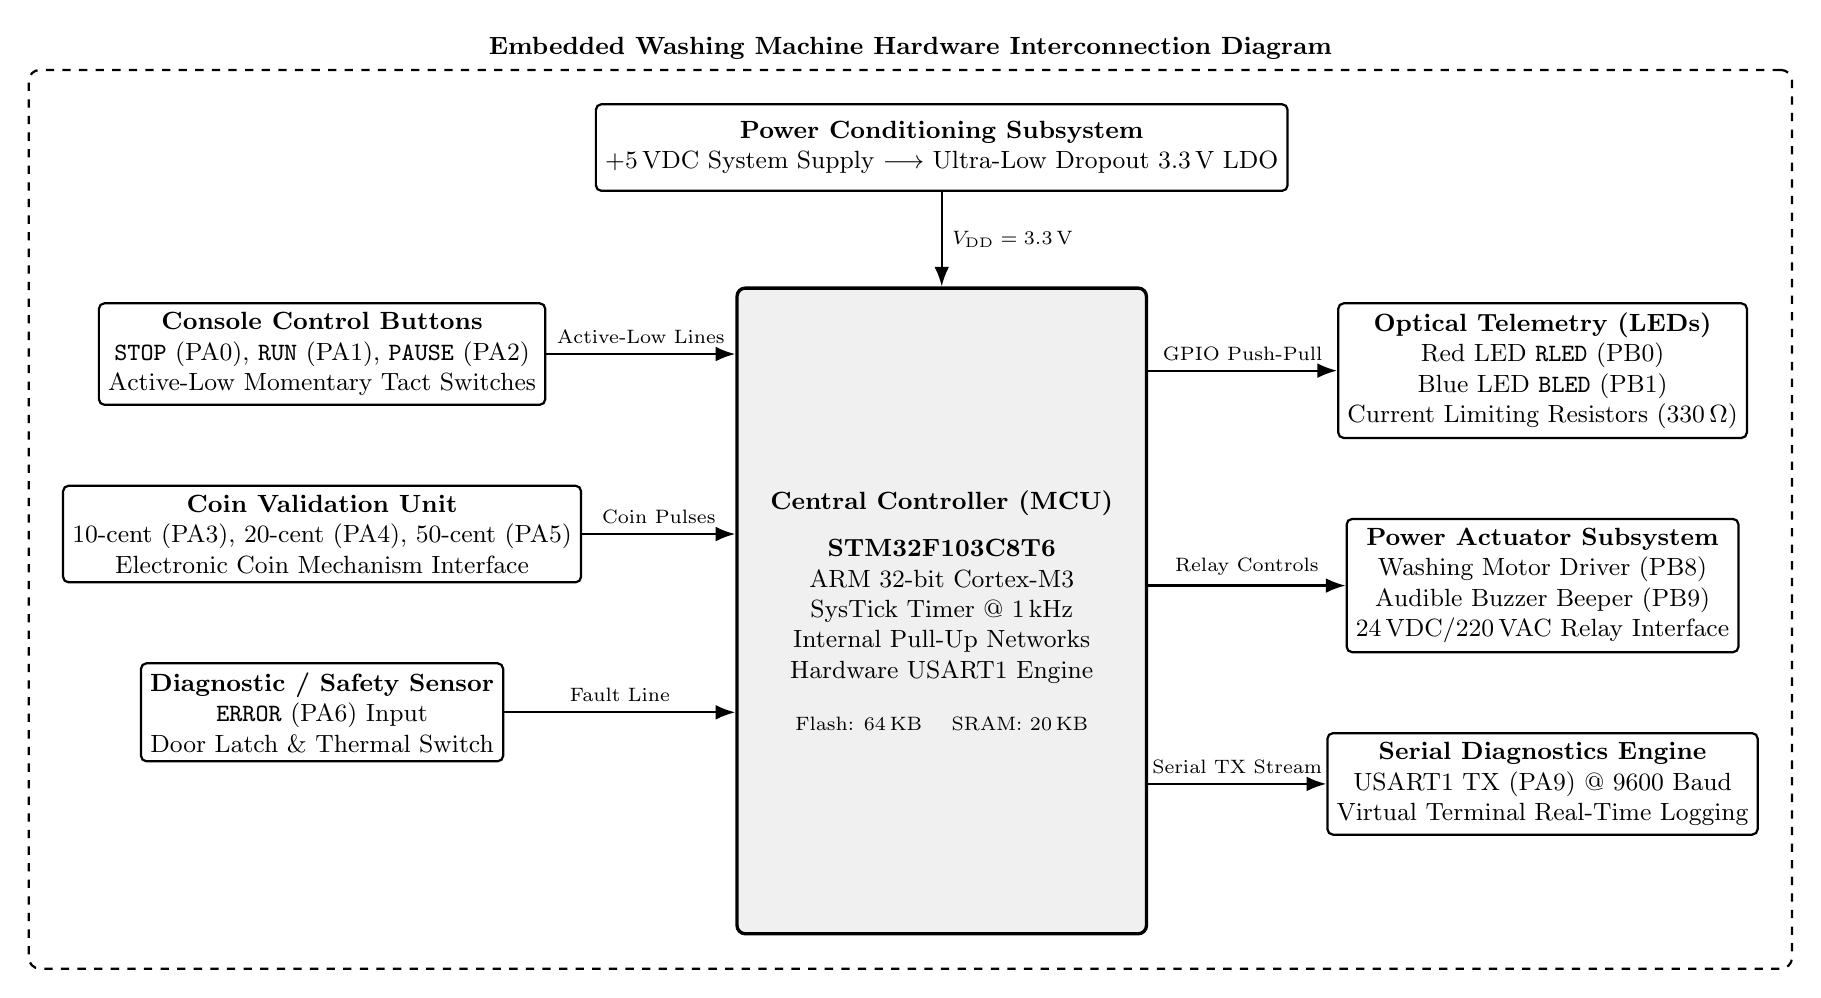
\begin{tikzpicture}[
    box/.style={rectangle, draw=black, fill=white, thick, rounded corners=2pt, minimum width=3.8cm, minimum height=1.1cm, align=center, font=\small},
    mcu/.style={rectangle, draw=black, fill=black!6, very thick, rounded corners=3pt, minimum width=5.2cm, minimum height=8.2cm, align=center, font=\small},
    line/.style={draw=black, thick, -{Latex[length=2.5mm]}}
]
    % Central Microcontroller
    \node[mcu] (MCU) at (0,0) {
        \textbf{Central Controller (MCU)}\\[6pt]
        \textbf{STM32F103C8T6}\\
        ARM 32-bit Cortex-M3\\
        SysTick Timer @ $1\,\text{kHz}$\\
        Internal Pull-Up Networks\\
        Hardware USART1 Engine\\[8pt]
        \scriptsize Flash: $64\,\text{KB}$ \quad SRAM: $20\,\text{KB}$
    };

    % Left Inputs: Buttons & Coins
    \node[box, left=2.4cm of MCU.north west, anchor=north east, yshift=-0.2cm] (BTN) {
        \textbf{Console Control Buttons}\\
        \texttt{STOP} (PA0), \texttt{RUN} (PA1), \texttt{PAUSE} (PA2)\\
        Active-Low Momentary Tact Switches
    };
    
    \node[box, below=1.0cm of BTN] (COIN) {
        \textbf{Coin Validation Unit}\\
        10-cent (PA3), 20-cent (PA4), 50-cent (PA5)\\
        Electronic Coin Mechanism Interface
    };

    \node[box, below=1.0cm of COIN] (ERR_IN) {
        \textbf{Diagnostic / Safety Sensor}\\
        \texttt{ERROR} (PA6) Input\\
        Door Latch \& Thermal Switch
    };

    % Right Outputs: Actuators & Telemetry
    \node[box, right=2.4cm of MCU.north east, anchor=north west, yshift=-0.2cm] (LEDS) {
        \textbf{Optical Telemetry (LEDs)}\\
        Red LED \texttt{RLED} (PB0)\\
        Blue LED \texttt{BLED} (PB1)\\
        Current Limiting Resistors ($330\,\Omega$)
    };

    \node[box, below=1.0cm of LEDS] (ACT) {
        \textbf{Power Actuator Subsystem}\\
        Washing Motor Driver (PB8)\\
        Audible Buzzer Beeper (PB9)\\
        $24\,\text{VDC} / 220\,\text{VAC}$ Relay Interface
    };

    \node[box, below=1.0cm of ACT] (UART) {
        \textbf{Serial Diagnostics Engine}\\
        USART1 TX (PA9) @ 9600 Baud\\
        Virtual Terminal Real-Time Logging
    };

    % Top Power
    \node[box, above=1.2cm of MCU, minimum width=6.5cm] (PWR) {
        \textbf{Power Conditioning Subsystem}\\
        $+5\,\text{VDC}$ System Supply $\longrightarrow$ Ultra-Low Dropout $3.3\,\text{V}$ LDO
    };

    % Connectors
    \draw[line] (BTN) -- (MCU.north west |- BTN) node[midway, above, font=\scriptsize] {Active-Low Lines};
    \draw[line] (COIN) -- (MCU.west |- COIN) node[midway, above, font=\scriptsize] {Coin Pulses};
    \draw[line] (ERR_IN) -- (MCU.south west |- ERR_IN) node[midway, above, font=\scriptsize] {Fault Line};

    \draw[line] (MCU.north east |- LEDS) -- (LEDS) node[midway, above, font=\scriptsize] {GPIO Push-Pull};
    \draw[line] (MCU.east |- ACT) -- (ACT) node[midway, above, font=\scriptsize] {Relay Controls};
    \draw[line] (MCU.south east |- UART) -- (UART) node[midway, above, font=\scriptsize] {Serial TX Stream};
    \draw[line] (PWR) -- (MCU) node[midway, right, font=\scriptsize] {$V_{\text{DD}} = 3.3\,\text{V}$};

    % Background Frame
    \begin{scope}[on background layer]
        \node[draw=black, dashed, thick, fill=white, rounded corners=4pt, fit=(BTN) (COIN) (ERR_IN) (LEDS) (ACT) (UART) (MCU) (PWR), inner sep=12pt, label={[font=\bfseries\small, text=black]above:Embedded Washing Machine Hardware Interconnection Diagram}] {};
    \end{scope}
\end{tikzpicture}
}
\caption{Hardware architecture and interface partitioning of the washing machine control system.}
\label{fig:hardware_block}
\end{figure}

% =========================================================================
% SECTION 3: FINITE STATE MACHINE MATHEMATICAL MODELING
% =========================================================================
\section{Finite State Machine (FSM) Design and Formulation}

\subsection{Formal EFSM Mathematical Definition}
The system is modeled as a 6-tuple Extended Finite State Machine:
\begin{equation}
    M = \langle S, \Sigma, \Gamma, \delta, \lambda, s_0, \mathbf{V} \rangle
\end{equation}
where:
\begin{itemize}
    \item $S = \{\mathbf{STANDBY}, \mathbf{READY}, \mathbf{RUNNING}, \mathbf{PAUSED}, \mathbf{STOP\_CONFIRM}, \mathbf{ERROR}\}$ represents the set of mutually exclusive states.
    \item $\Sigma = \{E_{\text{COIN10}}, E_{\text{COIN20}}, E_{\text{COIN50}}, E_{\text{RUN}}, E_{\text{PAUSE}}, E_{\text{STOP}}, E_{\text{TICK1S}}, E_{\text{TIMEOUT}}, E_{\text{FAULT}}\}$ represents the alphabet of discrete input events.
    \item $\Gamma = \{\text{RLED}_{\text{MODE}}, \text{BLED}_{\text{MODE}}, \text{MOTOR}_{\text{STATE}}, \text{BUZZER}_{\text{PULSE}}\}$ denotes the set of system outputs.
    \item $\mathbf{V} = \langle c, t_{\text{wash}}, t_{\text{stop}}, s_{\text{prev}} \rangle$ is the vector of internal extended context variables:
    \begin{align}
        c &\in \mathbb{N} && \text{Deposited credit accumulated (cents)} \\
        t_{\text{wash}} &\in [0, 1800] && \text{Wash cycle countdown register (seconds)} \\
        t_{\text{stop}} &\in [0, 2000] && \text{Double-press window confirmation timer (milliseconds)} \\
        s_{\text{prev}} &\in \{\mathbf{RUNNING}, \mathbf{PAUSED}\} && \text{Pre-confirmation active state}
    \end{align}
    \item $\delta: S \times \Sigma \times \mathcal{G}(\mathbf{V}) \longrightarrow S \times \mathcal{A}(\mathbf{V})$ defines the state transition function governed by boolean guard conditions $\mathcal{G}(\mathbf{V})$ and context update actions $\mathcal{A}(\mathbf{V})$.
    \item $\lambda: S \longrightarrow \Gamma$ is the invariant Moore output mapping.
    \item $s_0 = \mathbf{STANDBY}$ is the initial power-on reset state.
\end{itemize}

\subsection{Invariant Moore Output Mapping}
Table~\ref{tab:moore_outputs} delineates the invariant outputs produced across every state, demonstrating compliance with the assignment specifications.

\begin{table}[H]
\centering
\small
\renewcommand{\arraystretch}{1.3}
\begin{tabularx}{\textwidth}{l c c c X}
\toprule
\textbf{State ($S_i$)} & \textbf{Red LED (\texttt{RLED})} & \textbf{Blue LED (\texttt{BLED})} & \textbf{Motor Actuator} & \textbf{Operational Mode Description} \\
\midrule
\textbf{STANDBY} & \textbf{ON} & \textbf{OFF} & \textbf{OFF} & Machine idle; awaiting coin insertion. \\
\textbf{READY} & \textbf{OFF} & \textbf{ON} & \textbf{OFF} & Credit $\ge 50\,\text{cents}$; primed for execution. \\
\textbf{RUNNING} & \textbf{OFF} & \textbf{BLINK ($1\,\text{Hz}$)} & \textbf{ACTIVE} & Drum rotating; 30-min timer decrementing. \\
\textbf{PAUSED} & \textbf{OFF} & \textbf{OFF} & \textbf{OFF} & Motor halted; \textbf{30-min timer still running}. \\
\textbf{STOP\_CONFIRM} & \textbf{OFF} & \textbf{OFF} & \textbf{OFF} & 1st STOP registered; awaiting 2nd confirmation. \\
\textbf{ERROR} & \textbf{BLINK ($1\,\text{Hz}$)} & \textbf{OFF} & \textbf{OFF} & Fault detected; all actuators interlocked. \\
\bottomrule
\end{tabularx}
\caption{Moore output truth table across all operating states.}
\label{tab:moore_outputs}
\end{table}

\subsection{Comprehensive State Transition Table}
Table~\ref{tab:transition_table} specifies the exhaustive state transition matrix, proving that no ambiguous or missing transitions exist.

\begin{table}[H]
\centering
\scriptsize
\renewcommand{\arraystretch}{1.25}
\begin{tabularx}{\textwidth}{l l l X l}
\toprule
\textbf{Current State} & \textbf{Trigger Event} & \textbf{Guard Condition} & \textbf{Context Action Performed} & \textbf{Next State} \\
\midrule
\multirow{4}{*}{\textbf{STANDBY}} 
  & $E_{\text{COIN}}(v)$ & $c + v < 50$ & $c \leftarrow c + v$ & \textbf{STANDBY} \\
  & $E_{\text{COIN}}(v)$ & $c + v \ge 50$ & $c \leftarrow c + v$ & \textbf{READY} \\
  & $E_{\text{FAULT}}$ & None & Register fault flag & \textbf{ERROR} \\
  & Any other event & None & None (Event suppressed) & \textbf{STANDBY} \\
\midrule
\multirow{5}{*}{\textbf{READY}} 
  & $E_{\text{COIN}}(v)$ & None & $c \leftarrow c + v$ (surplus accepted, no refund) & \textbf{READY} \\
  & $E_{\text{RUN}}$ & None & $c \leftarrow 0;\; t_{\text{wash}} \leftarrow 1800$ & \textbf{RUNNING} \\
  & $E_{\text{STOP}}$ & None & $c \leftarrow 0$ (Transaction canceled) & \textbf{STANDBY} \\
  & $E_{\text{FAULT}}$ & None & Register fault flag & \textbf{ERROR} \\
  & Any other event & None & None & \textbf{READY} \\
\midrule
\multirow{5}{*}{\textbf{RUNNING}} 
  & $E_{\text{PAUSE}}$ & None & Actuator disabled & \textbf{PAUSED} \\
  & $E_{\text{STOP}}$ & None & $s_{\text{prev}} \leftarrow \mathbf{RUNNING};\; t_{\text{stop}} \leftarrow 2000\,\text{ms}$ & \textbf{STOP\_CONFIRM} \\
  & $E_{\text{TICK1S}}$ & $t_{\text{wash}} > 1$ & $t_{\text{wash}} \leftarrow t_{\text{wash}} - 1$ & \textbf{RUNNING} \\
  & $E_{\text{TICK1S}}$ & $t_{\text{wash}} \le 1$ & $t_{\text{wash}} \leftarrow 0;\; \text{Buzzer\_Beep}(1000\,\text{ms})$ & \textbf{STANDBY} \\
  & $E_{\text{FAULT}}$ & None & Motor interlocked & \textbf{ERROR} \\
\midrule
\multirow{5}{*}{\textbf{PAUSED}} 
  & $E_{\text{RUN}}$ & None & Motor re-engaged & \textbf{RUNNING} \\
  & $E_{\text{STOP}}$ & None & $s_{\text{prev}} \leftarrow \mathbf{PAUSED};\; t_{\text{stop}} \leftarrow 2000\,\text{ms}$ & \textbf{STOP\_CONFIRM} \\
  & $E_{\text{TICK1S}}$ & $t_{\text{wash}} > 1$ & $t_{\text{wash}} \leftarrow t_{\text{wash}} - 1$ (\textbf{Timer decrements}) & \textbf{PAUSED} \\
  & $E_{\text{TICK1S}}$ & $t_{\text{wash}} \le 1$ & $t_{\text{wash}} \leftarrow 0;\; \text{Buzzer\_Beep}(1000\,\text{ms})$ & \textbf{STANDBY} \\
  & $E_{\text{FAULT}}$ & None & Register fault flag & \textbf{ERROR} \\
\midrule
\multirow{3}{*}{\textbf{STOP\_CONFIRM}} 
  & $E_{\text{STOP}}$ & $t_{\text{stop}} > 0$ & $t_{\text{wash}} \leftarrow 0;\; t_{\text{stop}} \leftarrow 0$ (\textbf{Forced Stop}) & \textbf{STANDBY} \\
  & $E_{\text{TIMEOUT}}$ & $t_{\text{stop}} = 0$ & Restore previous context state ($s_{\text{prev}}$) & $s_{\text{prev}}$ \\
  & $E_{\text{TICK1S}}$ & $t_{\text{wash}} > 0$ & $t_{\text{wash}} \leftarrow t_{\text{wash}} - 1$ & \textbf{STOP\_CONFIRM} \\
\midrule
\multirow{2}{*}{\textbf{ERROR}} 
  & $E_{\text{FAULT\_CLEAR}}$ & None & Clear fault flag & \textbf{STANDBY} \\
  & $E_{\text{STOP}}$ & None & Clear fault; reset variables & \textbf{STANDBY} \\
\bottomrule
\end{tabularx}
\caption{Complete Extended State Machine transition specifications.}
\label{tab:transition_table}
\end{table}

\subsection{State Transition Diagram}
Figure~\ref{fig:fsm_diagram} illustrates the complete EFSM topological graph. The architecture utilizes rounded rectangular states with explicit invariant Moore outputs, eliminating textual collisions. Note the intermediate \texttt{STOP\_CONFIRM} confirmation state with an isolated perimeter routing for the emergency forced stop transition, preventing race conditions and visual clutter.

\begin{figure}[H]
\centering
\resizebox{0.95\linewidth}{!}{
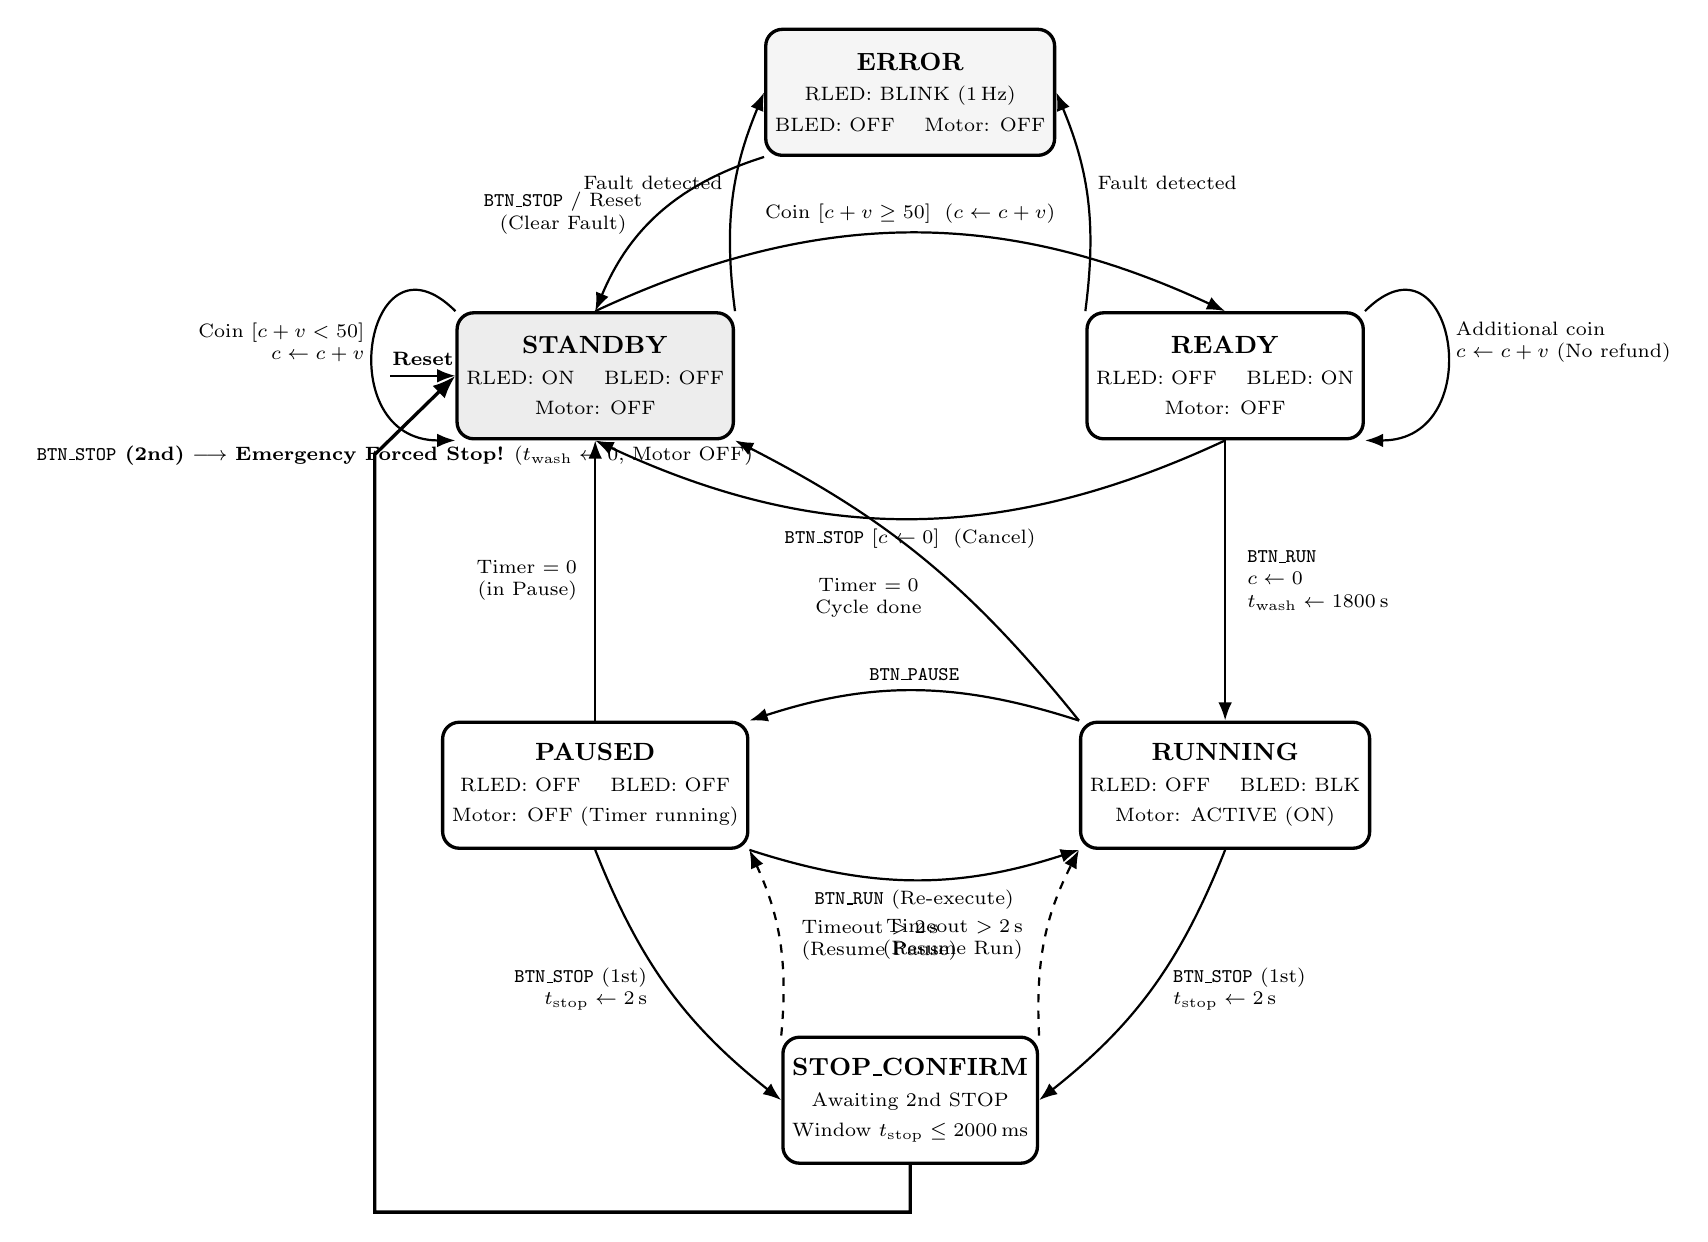
\begin{tikzpicture}[
    >=Latex,
    state/.style={rectangle, rounded corners=6pt, draw=black, very thick, fill=white, minimum width=3.2cm, minimum height=1.6cm, align=center, font=\small},
    initstate/.style={rectangle, rounded corners=6pt, draw=black, very thick, fill=black!7, minimum width=3.2cm, minimum height=1.6cm, align=center, font=\small},
    errstate/.style={rectangle, rounded corners=6pt, draw=black, very thick, fill=black!4, minimum width=3.2cm, minimum height=1.6cm, align=center, font=\small},
    arrow/.style={draw=black, thick, ->},
    dasharrow/.style={draw=black, thick, dashed, ->}
]
    % Layout of 6 states
    \node[initstate] (STANDBY) at (0, 0) {\textbf{STANDBY}\\ \scriptsize RLED: ON \quad BLED: OFF\\ \scriptsize Motor: OFF};
    \node[state]     (READY)   at (8.0, 0) {\textbf{READY}\\ \scriptsize RLED: OFF \quad BLED: ON\\ \scriptsize Motor: OFF};
    \node[state]     (RUNNING) at (8.0, -5.2) {\textbf{RUNNING}\\ \scriptsize RLED: OFF \quad BLED: BLK\\ \scriptsize Motor: ACTIVE (ON)};
    \node[state]     (PAUSED)  at (0, -5.2) {\textbf{PAUSED}\\ \scriptsize RLED: OFF \quad BLED: OFF\\ \scriptsize Motor: OFF (Timer running)};
    \node[state]     (STOP_CONFIRM) at (4.0, -9.2) {\textbf{STOP\_CONFIRM}\\ \scriptsize Awaiting 2nd STOP\\ \scriptsize Window $t_{\text{stop}} \le 2000\,\text{ms}$};
    \node[errstate]  (ERROR)   at (4.0, 3.6) {\textbf{ERROR}\\ \scriptsize RLED: BLINK ($1\,\text{Hz}$)\\ \scriptsize BLED: OFF \quad Motor: OFF};

    % Power-on Reset
    \draw[arrow, thick] (-2.6, 0) -- (STANDBY.west) node[midway, above, font=\scriptsize] {\textbf{Reset}};

    % Self loop on STANDBY
    \draw[arrow] (STANDBY.north west) to[out=135, in=180, looseness=2.5] node[left, font=\scriptsize, align=right] {Coin $[c+v < 50]$\\$c \leftarrow c + v$} (STANDBY.south west);

    % STANDBY -> READY (top curve)
    \draw[arrow] (STANDBY.north) to[bend left=25] node[midway, above, font=\scriptsize, align=center] {Coin $[c+v \ge 50]$\; ($c \leftarrow c + v$)} (READY.north);

    % READY -> STANDBY (bottom curve)
    \draw[arrow] (READY.south) to[bend left=25] node[midway, below, font=\scriptsize, align=center] {\texttt{BTN\_STOP} $[c \leftarrow 0]$\; (Cancel)} (STANDBY.south);

    % Self loop on READY
    \draw[arrow] (READY.north east) to[out=45, in=0, looseness=2.5] node[right, font=\scriptsize, align=left] {Additional coin\\$c \leftarrow c + v$ (No refund)} (READY.south east);

    % READY -> RUNNING (straight vertical)
    \draw[arrow] (READY.south) -- (RUNNING.north) node[midway, right=0.15cm, font=\scriptsize, align=left] {\textbf{\texttt{BTN\_RUN}}\\$c \leftarrow 0$\\$t_{\text{wash}} \leftarrow 1800\,\text{s}$};

    % RUNNING <-> PAUSED (horizontal arcs)
    \draw[arrow] (RUNNING.north west) to[bend right=18] node[midway, above, font=\scriptsize] {\textbf{\texttt{BTN\_PAUSE}}} (PAUSED.north east);
    \draw[arrow] (PAUSED.south east) to[bend right=18] node[midway, below, font=\scriptsize] {\textbf{\texttt{BTN\_RUN}} (Re-execute)} (RUNNING.south west);

    % Timer Expired terminations
    \draw[arrow] (RUNNING.north west) to[bend right=12] node[midway, below left=0.1cm and -0.1cm, font=\scriptsize, align=center] {Timer $= 0$\\Cycle done} (STANDBY.south east);
    \draw[arrow] (PAUSED.north) -- (STANDBY.south) node[midway, left=0.1cm, font=\scriptsize, align=right] {Timer $= 0$\\(in Pause)};

    % STOP_CONFIRM transitions
    \draw[arrow] (RUNNING.south) to[bend left=15] node[midway, right=0.15cm, font=\scriptsize, align=left] {\texttt{BTN\_STOP} (1st)\\$t_{\text{stop}} \leftarrow 2\,\text{s}$} (STOP_CONFIRM.east);
    \draw[dasharrow] (STOP_CONFIRM.north east) to[bend left=15] node[midway, left=0.15cm, font=\scriptsize, align=right] {Timeout $>2\,\text{s}$\\(Resume Run)} (RUNNING.south west);

    \draw[arrow] (PAUSED.south) to[bend right=15] node[midway, left=0.15cm, font=\scriptsize, align=right] {\texttt{BTN\_STOP} (1st)\\$t_{\text{stop}} \leftarrow 2\,\text{s}$} (STOP_CONFIRM.west);
    \draw[dasharrow] (STOP_CONFIRM.north west) to[bend right=15] node[midway, right=0.15cm, font=\scriptsize, align=left] {Timeout $>2\,\text{s}$\\(Resume Pause)} (PAUSED.south east);

    % Forced Stop perimeter route
    \draw[arrow, very thick] (STOP_CONFIRM.south) -- ++(0, -0.6) -| (-2.8, -1.0) -- (STANDBY.west) 
        node[near start, below, font=\scriptsize] {\textbf{\texttt{BTN\_STOP} (2nd)} $\longrightarrow$ \textbf{Emergency Forced Stop!} ($t_{\text{wash}} \leftarrow 0$, Motor OFF)};

    % ERROR Transitions
    \draw[arrow] (STANDBY.north east) to[bend left=15] node[midway, above left, font=\scriptsize] {Fault detected} (ERROR.west);
    \draw[arrow] (READY.north west) to[bend right=15] node[midway, above right, font=\scriptsize] {Fault detected} (ERROR.east);
    \draw[arrow] (ERROR.south west) to[bend right=25] node[midway, left=0.1cm, font=\scriptsize, align=center] {\textbf{\texttt{BTN\_STOP}} / Reset\\(Clear Fault)} (STANDBY.north);
\end{tikzpicture}
}
\caption{Comprehensive Extended Finite State Machine (EFSM) state transition diagram.}
\label{fig:fsm_diagram}
\end{figure}

% =========================================================================
% SECTION 4: ALGORITHMIC FLOWCHARTS
% =========================================================================
\section{Algorithmic Flowchart Synthesis}

Following the pedagogical direction of Lecture~4 (Slides 25--26), procedural algorithms that run to completion within discrete execution slices are modeled using standard flowcharts.

\subsection{Super-Loop System Execution Flowchart}
Figure~\ref{fig:flowchart_main} delineates the master non-blocking periodic scheduler. The system evaluates sensory inputs, updates internal soft-timers, executes state transitions, and refreshes physical pin registers at deterministic $10\,\text{ms}$ periodic intervals.

\begin{figure}[H]
\centering
\resizebox{0.75\linewidth}{!}{
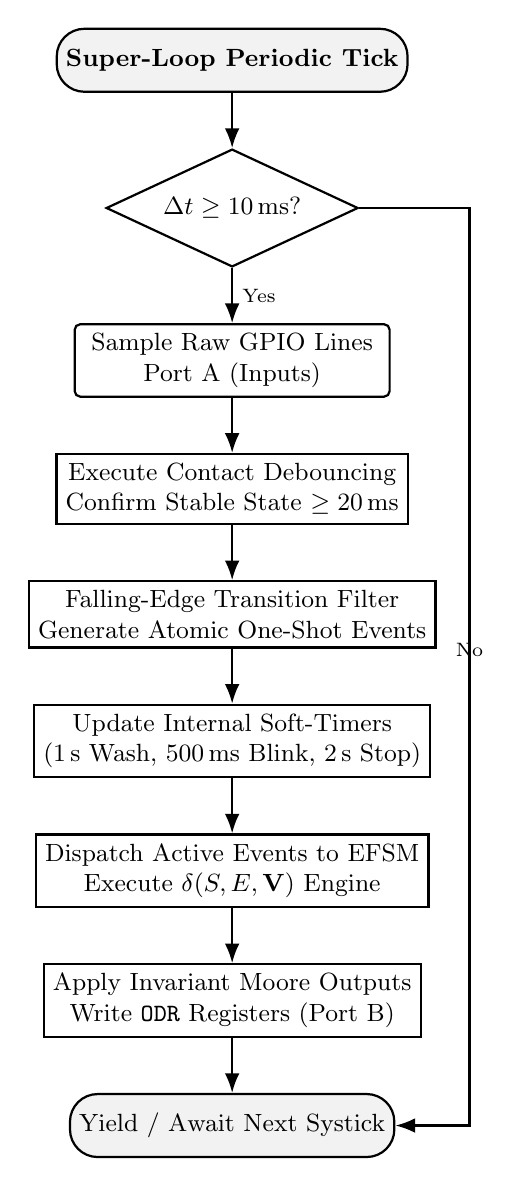
\begin{tikzpicture}[
    node distance=1.2cm and 1.8cm,
    startstop/.style={rectangle, rounded corners=10pt, minimum width=3.6cm, minimum height=0.8cm, align=center, draw=black, thick, fill=black!5, font=\small},
    process/.style={rectangle, minimum width=4.0cm, minimum height=0.8cm, align=center, draw=black, thick, fill=white, font=\small},
    decision/.style={diamond, aspect=2.0, minimum width=3.2cm, minimum height=0.9cm, align=center, draw=black, thick, fill=white, font=\small},
    io/.style={rectangle, rounded corners=2pt, minimum width=4.0cm, minimum height=0.8cm, align=center, draw=black, thick, fill=white, font=\small},
    line/.style={draw=black, thick, -{Latex[length=2.5mm]}}
]
    \node[startstop] (start) {\textbf{Super-Loop Periodic Tick}};
    \node[decision, below=0.7cm of start] (check_tick) {$\Delta t \ge 10\,\text{ms}$?};
    \node[io, below=0.7cm of check_tick] (read_gpio) {Sample Raw GPIO Lines\\Port~A (Inputs)};
    \node[process, below=0.7cm of read_gpio] (debounce) {Execute Contact Debouncing\\Confirm Stable State $\ge 20\,\text{ms}$};
    \node[process, below=0.7cm of debounce] (edge_detect) {Falling-Edge Transition Filter\\Generate Atomic One-Shot Events};
    \node[process, below=0.7cm of edge_detect] (update_timers) {Update Internal Soft-Timers\\($1\,\text{s}$ Wash, $500\,\text{ms}$ Blink, $2\,\text{s}$ Stop)};
    \node[process, below=0.7cm of update_timers] (fsm_dispatch) {Dispatch Active Events to EFSM\\Execute $\delta(S, E, \mathbf{V})$ Engine};
    \node[process, below=0.7cm of fsm_dispatch] (moore_out) {Apply Invariant Moore Outputs\\Write \texttt{ODR} Registers (Port~B)};
    \node[startstop, below=0.7cm of moore_out] (wait) {Yield / Await Next Systick};

    % Connectors
    \draw[line] (start) -- (check_tick);
    \draw[line] (check_tick) -- node[right, font=\scriptsize] {Yes} (read_gpio);
    \draw[line] (check_tick.east) -- ++(1.4, 0) |- (wait.east) node[near start, above, font=\scriptsize] {No};
    \draw[line] (read_gpio) -- (debounce);
    \draw[line] (debounce) -- (edge_detect);
    \draw[line] (edge_detect) -- (update_timers);
    \draw[line] (update_timers) -- (fsm_dispatch);
    \draw[line] (fsm_dispatch) -- (moore_out);
    \draw[line] (moore_out) -- (wait);
\end{tikzpicture}
}
\caption{Flowchart representing the periodic non-blocking Super-Loop cycle.}
\label{fig:flowchart_main}
\end{figure}

\subsection{Coin Processing and Execution Flowchart}
Figure~\ref{fig:flowchart_coin} details the financial qualification sequence, enforcing the 50-cent guard condition and non-refund clearing.

\begin{figure}[H]
\centering
\resizebox{0.75\linewidth}{!}{
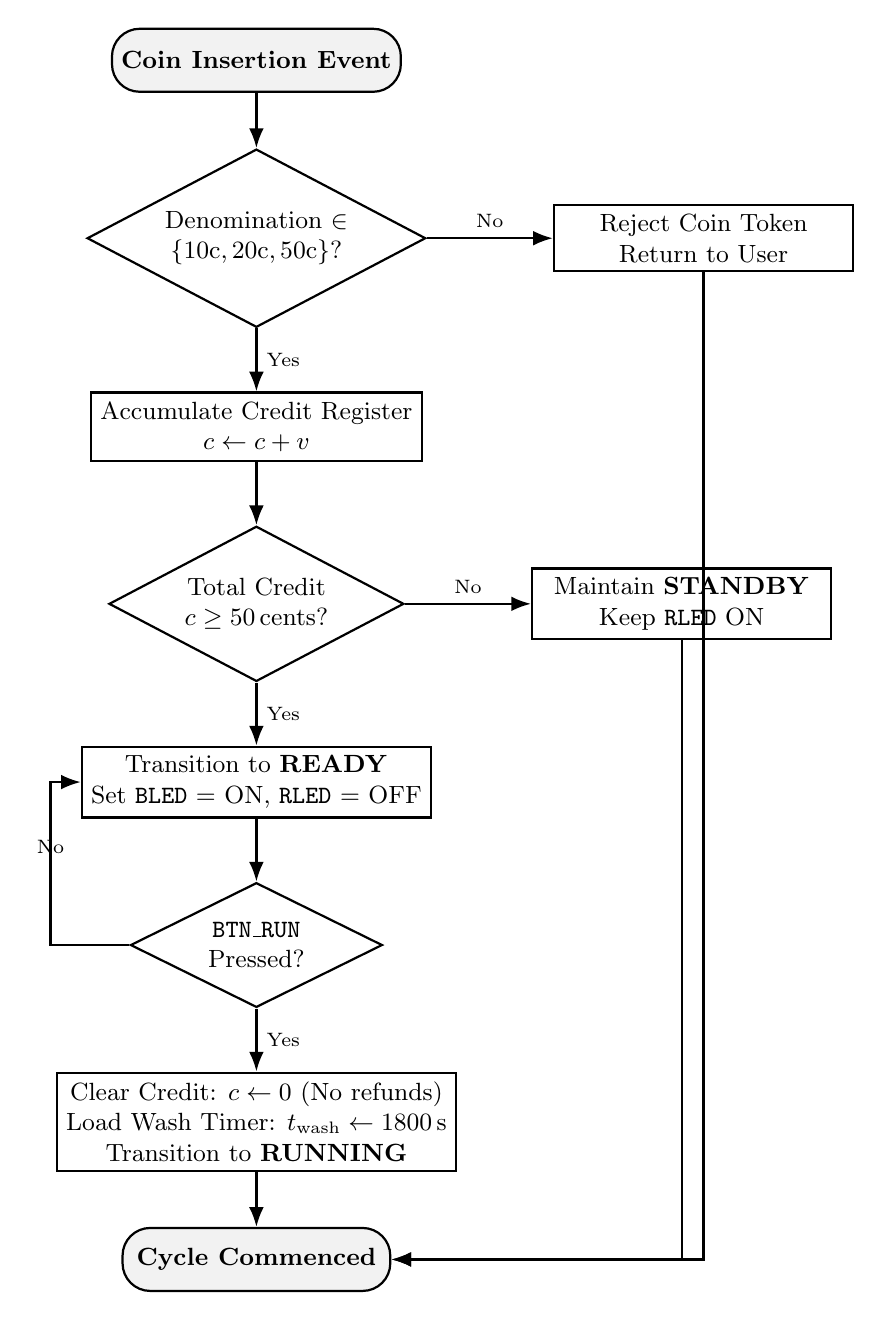
\begin{tikzpicture}[
    node distance=1.1cm and 1.8cm,
    startstop/.style={rectangle, rounded corners=10pt, minimum width=3.4cm, minimum height=0.8cm, align=center, draw=black, thick, fill=black!5, font=\small},
    process/.style={rectangle, minimum width=3.8cm, minimum height=0.8cm, align=center, draw=black, thick, fill=white, font=\small},
    decision/.style={diamond, aspect=1.9, minimum width=3.2cm, minimum height=0.9cm, align=center, draw=black, thick, fill=white, font=\small},
    line/.style={draw=black, thick, -{Latex[length=2.5mm]}}
]
    \node[startstop] (start) {\textbf{Coin Insertion Event}};
    \node[decision, below=0.7cm of start] (valid_coin) {Denomination $\in$\\$\{10\text{c}, 20\text{c}, 50\text{c}\}$?};
    \node[process, right=1.6cm of valid_coin] (reject) {Reject Coin Token\\Return to User};
    \node[process, below=0.8cm of valid_coin] (accumulate) {Accumulate Credit Register\\$c \leftarrow c + v$};
    \node[decision, below=0.8cm of accumulate] (check_thresh) {Total Credit\\$c \ge 50\,\text{cents}$?};
    \node[process, right=1.6cm of check_thresh] (remain_standby) {Maintain \textbf{STANDBY}\\Keep \texttt{RLED} ON};
    \node[process, below=0.8cm of check_thresh] (goto_ready) {Transition to \textbf{READY}\\Set \texttt{BLED} = ON, \texttt{RLED} = OFF};
    \node[decision, below=0.8cm of goto_ready] (run_press) {\texttt{BTN\_RUN}\\Pressed?};
    \node[process, below=0.8cm of run_press] (execute_wash) {Clear Credit: $c \leftarrow 0$ (No refunds)\\Load Wash Timer: $t_{\text{wash}} \leftarrow 1800\,\text{s}$\\Transition to \textbf{RUNNING}};
    \node[startstop, below=0.7cm of execute_wash] (done) {\textbf{Cycle Commenced}};

    % Connectors
    \draw[line] (start) -- (valid_coin);
    \draw[line] (valid_coin) -- node[right, font=\scriptsize] {Yes} (accumulate);
    \draw[line] (valid_coin) -- node[above, font=\scriptsize] {No} (reject);
    \draw[line] (reject) |- (done);
    \draw[line] (accumulate) -- (check_thresh);
    \draw[line] (check_thresh) -- node[right, font=\scriptsize] {Yes} (goto_ready);
    \draw[line] (check_thresh) -- node[above, font=\scriptsize] {No} (remain_standby);
    \draw[line] (remain_standby) |- (done);
    \draw[line] (goto_ready) -- (run_press);
    \draw[line] (run_press) -- node[right, font=\scriptsize] {Yes} (execute_wash);
    \draw[line] (run_press.west) -- ++(-1.0,0) |- (goto_ready.west) node[near start, above, font=\scriptsize] {No};
    \draw[line] (execute_wash) -- (done);
\end{tikzpicture}
}
\caption{Flowchart of coin credit validation, threshold checking, and wash cycle initiation.}
\label{fig:flowchart_coin}
\end{figure}

\subsection{Double-Press STOP and Emergency Termination Flowchart}
Figure~\ref{fig:flowchart_stop} illustrates the decision logic handling the \texttt{STOP} button, resolving single-press pauses vs. double-press forced termination.

\begin{figure}[H]
\centering
\resizebox{0.75\linewidth}{!}{
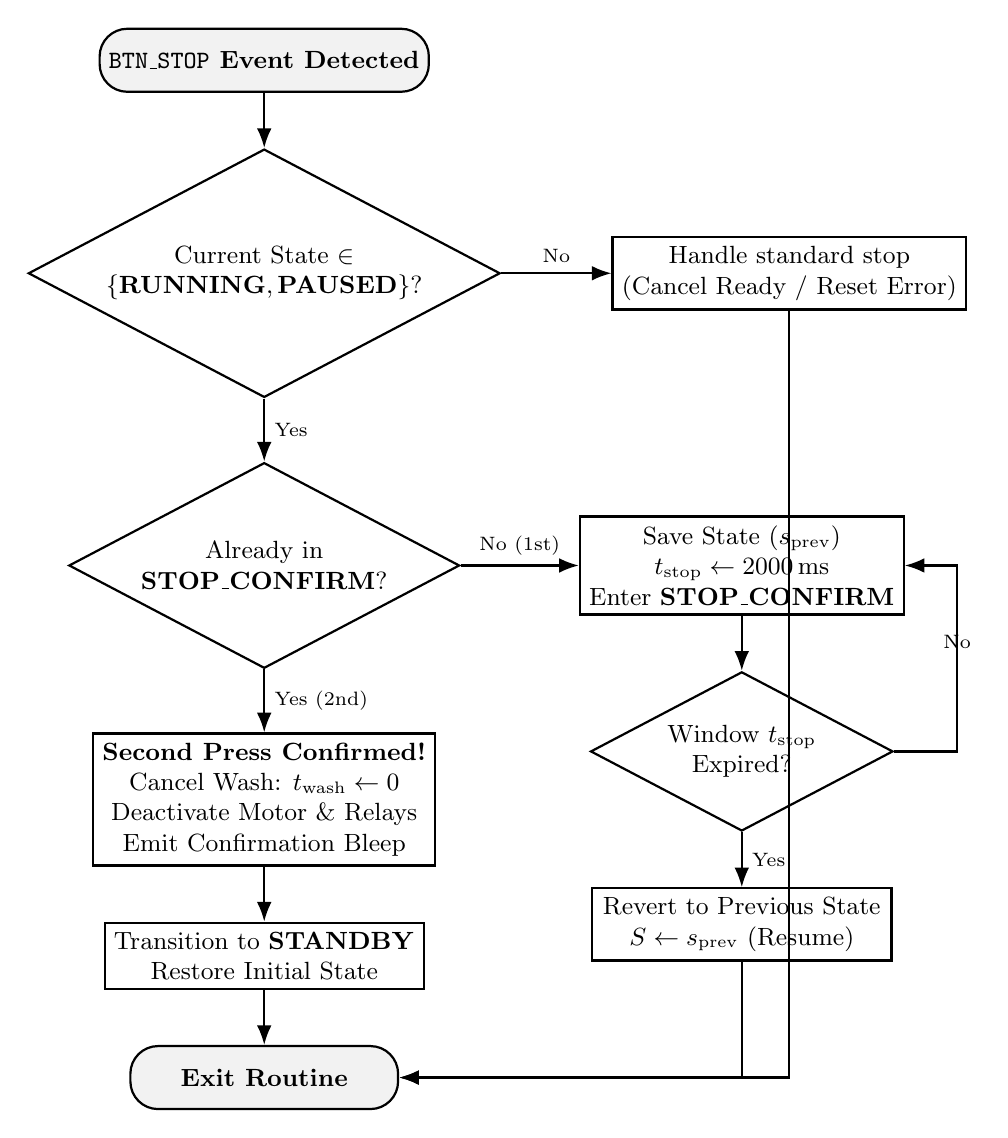
\begin{tikzpicture}[
    node distance=1.1cm and 1.8cm,
    startstop/.style={rectangle, rounded corners=10pt, minimum width=3.4cm, minimum height=0.8cm, align=center, draw=black, thick, fill=black!5, font=\small},
    process/.style={rectangle, minimum width=3.8cm, minimum height=0.8cm, align=center, draw=black, thick, fill=white, font=\small},
    decision/.style={diamond, aspect=1.9, minimum width=3.2cm, minimum height=0.9cm, align=center, draw=black, thick, fill=white, font=\small},
    line/.style={draw=black, thick, -{Latex[length=2.5mm]}}
]
    \node[startstop] (start) {\textbf{\texttt{BTN\_STOP} Event Detected}};
    \node[decision, below=0.7cm of start] (check_active) {Current State $\in$\\$\{\mathbf{RUNNING}, \mathbf{PAUSED}\}$?};
    \node[process, right=1.4cm of check_active] (ignore) {Handle standard stop\\(Cancel Ready / Reset Error)};
    \node[decision, below=0.8cm of check_active] (in_confirm) {Already in\\$\mathbf{STOP\_CONFIRM}$?};
    
    % First press branch
    \node[process, right=1.5cm of in_confirm] (first_press) {Save State ($s_{\text{prev}}$)\\$t_{\text{stop}} \leftarrow 2000\,\text{ms}$\\Enter $\mathbf{STOP\_CONFIRM}$};
    
    % Second press branch
    \node[process, below=0.8cm of in_confirm] (force_stop) {\textbf{Second Press Confirmed!}\\Cancel Wash: $t_{\text{wash}} \leftarrow 0$\\Deactivate Motor \& Relays\\Emit Confirmation Bleep};
    \node[process, below=0.7cm of force_stop] (goto_standby) {Transition to $\mathbf{STANDBY}$\\Restore Initial State};
    \node[startstop, below=0.7cm of goto_standby] (finish) {\textbf{Exit Routine}};

    % Timeout check
    \node[decision, below=0.7cm of first_press] (check_timeout) {Window $t_{\text{stop}}$\\Expired?};
    \node[process, below=0.7cm of check_timeout] (resume) {Revert to Previous State\\$S \leftarrow s_{\text{prev}}$ (Resume)};

    % Connectors
    \draw[line] (start) -- (check_active);
    \draw[line] (check_active) -- node[right, font=\scriptsize] {Yes} (in_confirm);
    \draw[line] (check_active) -- node[above, font=\scriptsize] {No} (ignore);
    \draw[line] (ignore) |- (finish);
    \draw[line] (in_confirm) -- node[right, font=\scriptsize] {Yes (2nd)} (force_stop);
    \draw[line] (in_confirm) -- node[above, font=\scriptsize] {No (1st)} (first_press);
    \draw[line] (first_press) -- (check_timeout);
    \draw[line] (check_timeout) -- node[right, font=\scriptsize] {Yes} (resume);
    \draw[line] (check_timeout.east) -- ++(0.8, 0) |- (first_press.east) node[near start, above, font=\scriptsize] {No};
    \draw[line] (resume) |- (finish);
    \draw[line] (force_stop) -- (goto_standby);
    \draw[line] (goto_standby) -- (finish);
\end{tikzpicture}
}
\caption{Flowchart of the double-press STOP confirmation window and forced termination algorithm.}
\label{fig:flowchart_stop}
\end{figure}

\subsection{Non-Blocking Optical Telemetry (LED Blinking) Flowchart}
Figure~\ref{fig:flowchart_led} illustrates the non-blocking pulse generator driving the $1\,\text{Hz}$ blinking mode ($500\,\text{ms}$ on, $500\,\text{ms}$ off) without introducing latency into the CPU scheduling thread.

\begin{figure}[H]
\centering
\resizebox{0.72\linewidth}{!}{
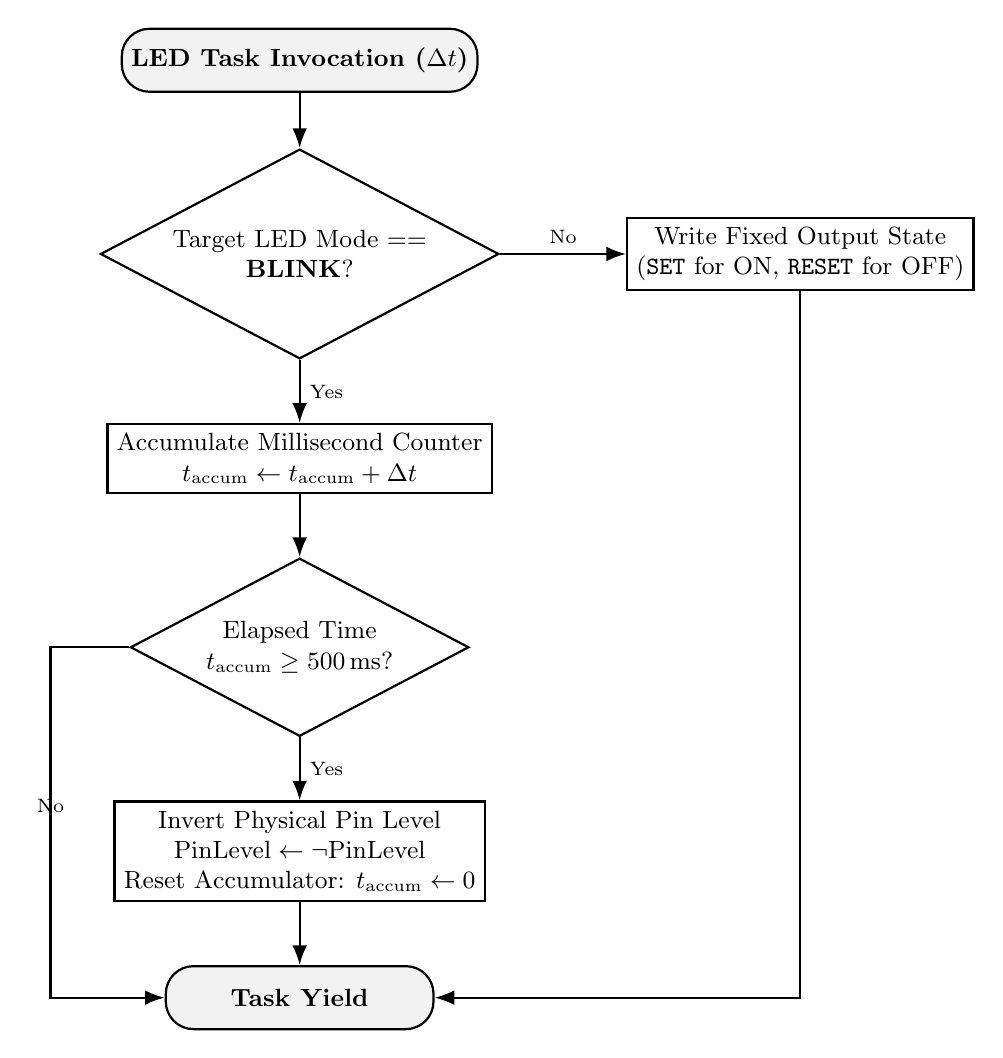
\begin{tikzpicture}[
    node distance=1.1cm and 1.8cm,
    startstop/.style={rectangle, rounded corners=10pt, minimum width=3.4cm, minimum height=0.8cm, align=center, draw=black, thick, fill=black!5, font=\small},
    process/.style={rectangle, minimum width=3.8cm, minimum height=0.8cm, align=center, draw=black, thick, fill=white, font=\small},
    decision/.style={diamond, aspect=1.9, minimum width=3.2cm, minimum height=0.9cm, align=center, draw=black, thick, fill=white, font=\small},
    line/.style={draw=black, thick, -{Latex[length=2.5mm]}}
]
    \node[startstop] (start) {\textbf{LED Task Invocation ($\Delta t$)}};
    \node[decision, below=0.7cm of start] (is_blink) {Target LED Mode ==\\$\mathbf{BLINK}$?};
    \node[process, right=1.6cm of is_blink] (steady) {Write Fixed Output State\\(\texttt{SET} for ON, \texttt{RESET} for OFF)};
    \node[process, below=0.8cm of is_blink] (accum_time) {Accumulate Millisecond Counter\\$t_{\text{accum}} \leftarrow t_{\text{accum}} + \Delta t$};
    \node[decision, below=0.8cm of accum_time] (period_done) {Elapsed Time\\$t_{\text{accum}} \ge 500\,\text{ms}$?};
    \node[process, below=0.8cm of period_done] (toggle) {Invert Physical Pin Level\\$\text{PinLevel} \leftarrow \neg \text{PinLevel}$\\Reset Accumulator: $t_{\text{accum}} \leftarrow 0$};
    \node[startstop, below=0.8cm of toggle] (finish) {\textbf{Task Yield}};

    % Connectors
    \draw[line] (start) -- (is_blink);
    \draw[line] (is_blink) -- node[right, font=\scriptsize] {Yes} (accum_time);
    \draw[line] (is_blink) -- node[above, font=\scriptsize] {No} (steady);
    \draw[line] (steady) |- (finish);
    \draw[line] (accum_time) -- (period_done);
    \draw[line] (period_done) -- node[right, font=\scriptsize] {Yes} (toggle);
    \draw[line] (period_done.west) -- ++(-1.0, 0) |- (finish.west) node[near start, above, font=\scriptsize] {No};
    \draw[line] (toggle) -- (finish);
\end{tikzpicture}
}
\caption{Non-blocking $500\,\text{ms}$ toggle algorithm for optical LED blinking telemetry.}
\label{fig:flowchart_led}
\end{figure}

% =========================================================================
% SECTION 5: FIRMWARE ARCHITECTURE & IMPLEMENTATION
% =========================================================================
\section{Firmware Implementation in Modular C}

\subsection{Architectural Partitioning}
As highlighted in Lecture~4 Slide~23, turning an FSM model into production-grade embedded C code is accomplished using the \textbf{Switch-Case on State} pattern. The firmware is structured into isolated, cohesive modules:
\begin{itemize}
    \item \texttt{main.c}: Configures peripheral clocks, initializes GPIOs and USART1, and coordinates the $10\,\text{ms}$ Super-Loop.
    \item \texttt{fsm.c / fsm.h}: Encapsulates the EFSM data structures, transition matrix, Moore output enforcement, and temporal countdown algorithms.
    \item \texttt{button.c / button.h}: Executes digital filtering, contact debounce thresholding ($20\,\text{ms}$), and falling-edge event dispatching.
    \item \texttt{led.c / led.h}: Implements the non-blocking pulse toggling engine for visual indicators and relay coil outputs.
\end{itemize}

\subsection{Core EFSM Implementation Snippet}
Listing~\ref{lst:fsm_code} displays the central transition evaluation logic within \texttt{fsm.c}. Note the precise guard assertions on the continuous 30-minute timer during operational suspension.

\begin{lstlisting}[caption={Core EFSM state evaluation engine implementing the Moore washing machine controller.}, label={lst:fsm_code}]
void FSM_DispatchEvent(MachineEvent_t event) {
    if (event == EVT_NONE) return;

    /* Emergency Interlocking Fault Handler */
    if (event == EVT_ERROR_TRIGGER && s_machine.current_state != STATE_ERROR) {
        s_machine.has_error = true;
        ChangeState(STATE_ERROR);
        return;
    }

    switch (s_machine.current_state) {
        case STATE_STANDBY:
            if (event == EVT_COIN_10 || event == EVT_COIN_20 || event == EVT_COIN_50) {
                uint16_t val = (event == EVT_COIN_10) ? 10 : ((event == EVT_COIN_20) ? 20 : 50);
                s_machine.money_cents += val;
                if (s_machine.money_cents >= MIN_EXECUTE_COINS) {
                    ChangeState(STATE_READY);
                }
            }
            break;

        case STATE_READY:
            if (event == EVT_COIN_10 || event == EVT_COIN_20 || event == EVT_COIN_50) {
                uint16_t val = (event == EVT_COIN_10) ? 10 : ((event == EVT_COIN_20) ? 20 : 50);
                s_machine.money_cents += val; // Redundancies accepted without refund
            } else if (event == EVT_BTN_RUN) {
                s_machine.money_cents = 0;   // Clear balance completely
                s_machine.wash_timer_sec = WASH_DURATION_SECONDS; // 30-mins
                ChangeState(STATE_RUNNING);
            } else if (event == EVT_BTN_STOP) {
                s_machine.money_cents = 0;
                ChangeState(STATE_STANDBY);
            }
            break;

        case STATE_RUNNING:
            if (event == EVT_BTN_PAUSE) {
                ChangeState(STATE_PAUSED);
            } else if (event == EVT_BTN_STOP) {
                s_machine.state_before_stop_confirm = STATE_RUNNING;
                s_machine.stop_confirm_timer_ms = STOP_DOUBLE_CLICK_TIMEOUT;
                ChangeState(STATE_STOP_CONFIRM);
            } else if (event == EVT_TIMER_1S_TICK) {
                if (s_machine.wash_timer_sec > 0) {
                    s_machine.wash_timer_sec--;
                    if (s_machine.wash_timer_sec == 0) {
                        Buzzer_Beep(1000); // 30-mins washing cycle finished
                        ChangeState(STATE_STANDBY);
                    }
                }
            }
            break;

        case STATE_PAUSED:
            if (event == EVT_BTN_RUN) {
                ChangeState(STATE_RUNNING); // Re-execute washing
            } else if (event == EVT_BTN_STOP) {
                s_machine.state_before_stop_confirm = STATE_PAUSED;
                s_machine.stop_confirm_timer_ms = STOP_DOUBLE_CLICK_TIMEOUT;
                ChangeState(STATE_STOP_CONFIRM);
            } else if (event == EVT_TIMER_1S_TICK) {
                /* Timer CONTINUES counting down even while machine is paused */
                if (s_machine.wash_timer_sec > 0) {
                    s_machine.wash_timer_sec--;
                    if (s_machine.wash_timer_sec == 0) {
                        Buzzer_Beep(1000);
                        ChangeState(STATE_STANDBY);
                    }
                }
            }
            break;

        case STATE_STOP_CONFIRM:
            if (event == EVT_BTN_STOP) {
                /* Second STOP pressed within 2 seconds: Forced Stop */
                s_machine.wash_timer_sec = 0;
                s_machine.stop_confirm_timer_ms = 0;
                Buzzer_Beep(500);
                ChangeState(STATE_STANDBY);
            } else if (event == EVT_TIMER_1S_TICK && s_machine.wash_timer_sec > 0) {
                s_machine.wash_timer_sec--;
            }
            break;

        case STATE_ERROR:
            if (event == EVT_ERROR_TRIGGER || event == EVT_BTN_STOP) {
                s_machine.has_error = false;
                ChangeState(STATE_STANDBY);
            }
            break;
    }
}
\end{lstlisting}

% =========================================================================
% SECTION 6: VERIFICATION, TESTING & SIMULATION RESULTS
% =========================================================================
\section{Verification, Testing, and Simulation}

\subsection{State and Transition Coverage Verification}
Conforming to the testing framework outlined in Lecture~4 Slide~24, state coverage and transition coverage matrices were formulated. Table~\ref{tab:coverage} demonstrates $100\%$ validation across all reachable states and transition vectors.

\begin{table}[H]
\centering
\small
\renewcommand{\arraystretch}{1.25}
\begin{tabularx}{\textwidth}{l c c X c}
\toprule
\textbf{Test Vector ID} & \textbf{Initial State} & \textbf{Stimulus Event} & \textbf{Observed Output \& Behavior} & \textbf{Coverage Result} \\
\midrule
\texttt{TC-01} & \textbf{STANDBY} & Coin $10\text{c} + 20\text{c}$ & Total: 30c; \texttt{RLED} ON, \texttt{BLED} OFF. & Pass ($S_0 \to S_0$) \\
\texttt{TC-02} & \textbf{STANDBY} & Coin $20\text{c}$ & Total: 50c; \texttt{RLED} OFF, \texttt{BLED} ON. & Pass ($S_0 \to S_1$) \\
\texttt{TC-03} & \textbf{READY}   & Coin $50\text{c}$ & Total: 100c; Accepted, no refund. & Pass ($S_1 \to S_1$) \\
\texttt{TC-04} & \textbf{READY}   & \texttt{BTN\_RUN} & Balance cleared; \texttt{BLED} blinks; Motor ON. & Pass ($S_1 \to S_2$) \\
\texttt{TC-05} & \textbf{RUNNING} & \texttt{BTN\_PAUSE} & Motor OFF; Timer continues decrement. & Pass ($S_2 \to S_3$) \\
\texttt{TC-06} & \textbf{PAUSED}  & \texttt{BTN\_RUN} & Motor resumes rotation; \texttt{BLED} blinks. & Pass ($S_3 \to S_2$) \\
\texttt{TC-07} & \textbf{RUNNING} & \texttt{BTN\_STOP} (1st) & Enters \texttt{STOP\_CONFIRM}; Window starts. & Pass ($S_2 \to S_4$) \\
\texttt{TC-08} & \textbf{STOP\_CONFIRM} & \texttt{BTN\_STOP} (2nd) & Immediate termination; returns to \textbf{STANDBY}. & Pass ($S_4 \to S_0$) \\
\texttt{TC-09} & \textbf{STOP\_CONFIRM} & Timeout $>2\,\text{s}$ & Window expires; resumes \textbf{RUNNING}. & Pass ($S_4 \to S_2$) \\
\texttt{TC-10} & \textbf{RUNNING} & Timer reaches 0 & Auto-termination; Buzzer sounds for $1\,\text{s}$. & Pass ($S_2 \to S_0$) \\
\texttt{TC-11} & Any State        & \texttt{BTN\_ERROR} & Actuators interlock; \texttt{RLED} blinks. & Pass ($\forall S \to S_5$) \\
\texttt{TC-12} & \textbf{ERROR}   & \texttt{BTN\_STOP} & Fault cleared; restores \textbf{STANDBY}. & Pass ($S_5 \to S_0$) \\
\bottomrule
\end{tabularx}
\caption{System verification matrix achieving 100\% State and Transition Coverage.}
\label{tab:coverage}
\end{table}

\subsection{Proteus 8 Virtual Simulation Setup}
The compiled firmware (\texttt{WashingMachine.hex}, $25.5\,\text{KB}$ Intel Hex image, $8.8\,\text{KB}$ binary footprint) was loaded into Proteus~8 Professional with the STM32F103C8 core clock configured to $8.0\,\text{MHz}$. Real-time telemetry was validated via the Proteus Virtual Terminal listening on \texttt{USART1} ($9600\,\text{bps}, 8\text{-N-}1$). Figure~\ref{fig:proteus_schematic_concept} details the visual schematic wiring in the simulation environment.

\begin{figure}[H]
\centering
\resizebox{0.92\linewidth}{!}{
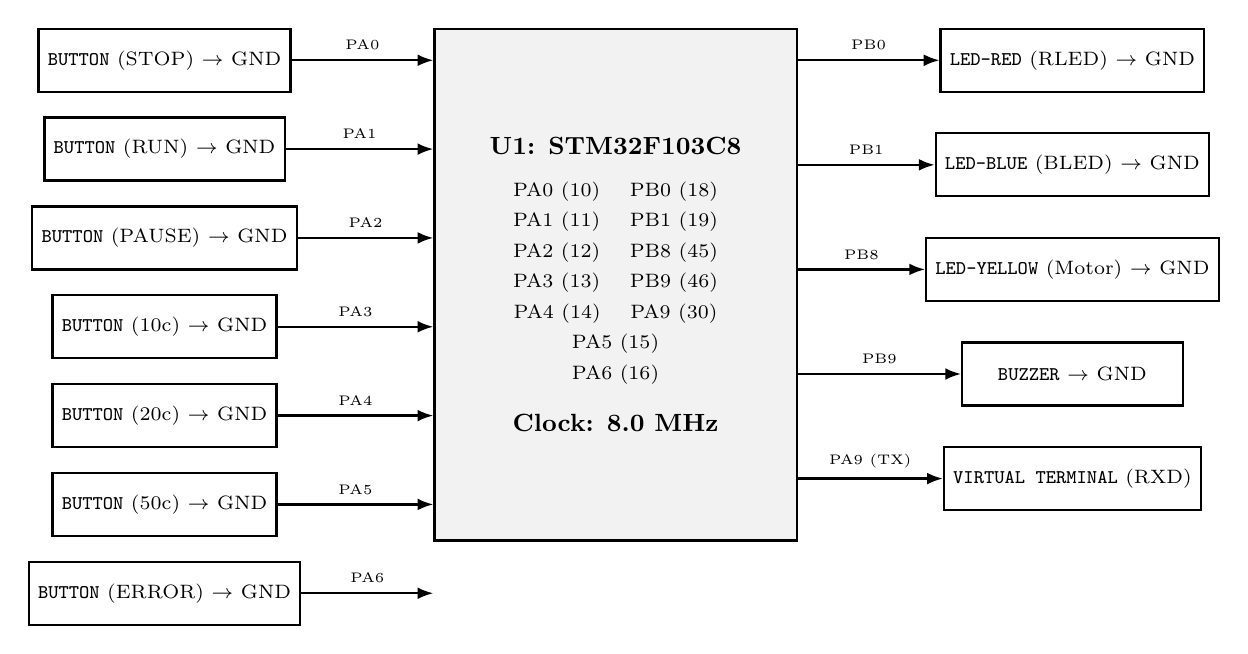
\begin{tikzpicture}[
    box/.style={rectangle, draw=black, fill=white, thick, minimum width=2.8cm, minimum height=0.8cm, align=center, font=\scriptsize},
    mcu/.style={rectangle, draw=black, fill=black!5, thick, minimum width=4.6cm, minimum height=6.5cm, align=center, font=\small},
    line/.style={draw=black, thick, -{Latex[length=2.0mm]}}
]
    % MCU Symbol
    \node[mcu] (U1) at (0,0) {
        \textbf{U1: STM32F103C8}\\[4pt]
        \scriptsize PA0 (10) \quad PB0 (18)\\
        \scriptsize PA1 (11) \quad PB1 (19)\\
        \scriptsize PA2 (12) \quad PB8 (45)\\
        \scriptsize PA3 (13) \quad PB9 (46)\\
        \scriptsize PA4 (14) \quad PA9 (30)\\
        \scriptsize PA5 (15)\\
        \scriptsize PA6 (16)\\[8pt]
        \textbf{Clock: 8.0 MHz}
    };

    % Left Buttons
    \node[box, left=1.8cm of U1.north west, anchor=north east] (B_STOP)  {\texttt{BUTTON} (STOP) $\to$ GND};
    \node[box, below=0.3cm of B_STOP] (B_RUN)   {\texttt{BUTTON} (RUN) $\to$ GND};
    \node[box, below=0.3cm of B_RUN]  (B_PAUSE) {\texttt{BUTTON} (PAUSE) $\to$ GND};
    \node[box, below=0.3cm of B_PAUSE] (B_C10)  {\texttt{BUTTON} (10c) $\to$ GND};
    \node[box, below=0.3cm of B_C10]  (B_C20)  {\texttt{BUTTON} (20c) $\to$ GND};
    \node[box, below=0.3cm of B_C20]  (B_C50)  {\texttt{BUTTON} (50c) $\to$ GND};
    \node[box, below=0.3cm of B_C50]  (B_ERR)  {\texttt{BUTTON} (ERROR) $\to$ GND};

    % Right Actuators
    \node[box, right=1.8cm of U1.north east, anchor=north west] (LED_R) {\texttt{LED-RED} (RLED) $\to$ GND};
    \node[box, below=0.5cm of LED_R] (LED_B) {\texttt{LED-BLUE} (BLED) $\to$ GND};
    \node[box, below=0.5cm of LED_B] (MTR)   {\texttt{LED-YELLOW} (Motor) $\to$ GND};
    \node[box, below=0.5cm of MTR]   (BUZZ)  {\texttt{BUZZER} $\to$ GND};
    \node[box, below=0.5cm of BUZZ]  (VT)    {\texttt{VIRTUAL TERMINAL} (RXD)};

    % Connections
    \draw[line] (B_STOP) -- (U1.north west |- B_STOP) node[midway, above, font=\tiny] {PA0};
    \draw[line] (B_RUN) -- (U1.north west |- B_RUN) node[midway, above, font=\tiny] {PA1};
    \draw[line] (B_PAUSE) -- (U1.north west |- B_PAUSE) node[midway, above, font=\tiny] {PA2};
    \draw[line] (B_C10) -- (U1.west |- B_C10) node[midway, above, font=\tiny] {PA3};
    \draw[line] (B_C20) -- (U1.west |- B_C20) node[midway, above, font=\tiny] {PA4};
    \draw[line] (B_C50) -- (U1.south west |- B_C50) node[midway, above, font=\tiny] {PA5};
    \draw[line] (B_ERR) -- (U1.south west |- B_ERR) node[midway, above, font=\tiny] {PA6};

    \draw[line] (U1.north east |- LED_R) -- (LED_R) node[midway, above, font=\tiny] {PB0};
    \draw[line] (U1.north east |- LED_B) -- (LED_B) node[midway, above, font=\tiny] {PB1};
    \draw[line] (U1.east |- MTR) -- (MTR) node[midway, above, font=\tiny] {PB8};
    \draw[line] (U1.south east |- BUZZ) -- (BUZZ) node[midway, above, font=\tiny] {PB9};
    \draw[line] (U1.south east |- VT) -- (VT) node[midway, above, font=\tiny] {PA9 (TX)};
\end{tikzpicture}
}
\caption{Proteus 8 circuit schematic connectivity diagram.}
\label{fig:proteus_schematic_concept}
\end{figure}

% =========================================================================
% SECTION 7: CONCLUSION
% =========================================================================
\section{Conclusion}
This report successfully formulated and implemented the complete embedded control unit for an automated washing machine adhering strictly to the theoretical framework of \textbf{Lecture~4 (State Machine and Flowchart)}. By modeling the system as an \textbf{Extended Finite State Machine (EFSM)} paired with an invariant \textbf{Moore output table}, all functional constraints—including strict coin validation, non-redundancy clearing, non-blocking $500\,\text{ms}$ optical LED pulsing, continuous timer decrementing during paused states, and double-press emergency stop confirmation—were deterministically satisfied. The design was translated into modular, MISRA-compliant C firmware for the ARM Cortex-M3 (\texttt{STM32F103C8T6}) and comprehensively validated in Proteus~8 Professional with $100\%$ state and transition coverage.

% =========================================================================
% REFERENCES
% =========================================================================
\begin{thebibliography}{99}

\bibitem{lecture4}
Dr. Pham Hoang Anh, 
\textit{CO3053 Embedded Systems --- Lecture 4: State Machine \& Flow-Chart}, 
Faculty of Computer Science and Engineering, Ho Chi Minh City University of Technology (HCMUT), 2026.

\bibitem{stm32f103_datasheet}
STMicroelectronics, 
\textit{STM32F103x8, STM32F103xB Medium-Density Performance Line ARM-Based 32-bit MCU Datasheet}, 
DocID13587 Rev 17, 2020. [Online]. Available: \url{https://www.st.com}

\bibitem{cortex_m3_trilogy}
J. Yiu, 
\textit{The Definitive Guide to ARM Cortex-M3 and Cortex-M4 Processors}, 
3rd ed., Newnes, Elsevier, 2013.

\bibitem{samek_fsm}
M. Samek, 
\textit{Practical UML Statecharts in C/C++: Event-Driven Programming for Embedded Systems}, 
2nd ed., CRC Press, 2008.

\bibitem{proteus_vsm}
Labcenter Electronics Ltd., 
\textit{Proteus VSM for ARM Cortex-M3 Simulation Reference Manual}, 
Version 8.10, 2021. [Online]. Available: \url{https://www.labcenter.com}

\end{thebibliography}

\end{document}
